\chapter{ĐO ĐẠC VÀ KIỂM THỬ HỆ THỐNG}
\section{Môi trường và kịch bản kiểm thử}
Phần mềm được chạy trên Windows 11, Python 3.12.7, NumPy 2.4.4, scikit-learn 1.8.0; mã build dùng PlatformIO 6.2.0. Thời gian đo CPU dùng \code{time.perf_counter()}; lệnh và tuổi bản tin dùng timestamp của PC. Khi chưa có board USB, simulator thay adapter vật lý nhưng vẫn đi qua hàm ingest, command và ack bình thường.

\begin{longtable}{P{1.1cm}P{6.5cm}P{4.2cm}P{2.8cm}}
\caption{Kịch bản và phạm vi bằng chứng}\\
\toprule Mã & Kịch bản & Kết quả mong đợi & Phạm vi \\ \midrule
K01 & Gói hợp lệ, gói trùng, seq cũ và boot mới & Lưu đúng; bỏ trùng; nhận boot mới & Test phần mềm \\
K02 & NaN/Inf, độ ẩm ngoài miền, boolean sai kiểu, device lạ & Từ chối và không tạo reading/outbox & Test phần mềm \\
K03 & 27 $\rightarrow$ 32 $\rightarrow$ 31 $\rightarrow$ 30 °C & Một raised, giữ trạng thái giữa, một cleared & Test phần mềm \\
K04 & Gửi lệnh, ACK sai ID/giá trị rồi ACK đúng & Giữ pending đến ACK đúng & Test phần mềm \\
K05 & Không có ACK, ACK muộn, RPC lặp & Timeout không giả thành công; không áp dụng lặp & Test phần mềm \\
K06 & Publish thất bại và mở lại SQLite & Không mất 1.000 bản tin đã lưu & Benchmark local \\
K07 & HTTP điều khiển, CSV và cross-origin & 202 pending, xuất events, chặn Origin ngoài & Test HTTP thật \\
K08 & Serial chia gói, log boot và JSON sai & Ghép dòng, bỏ sai, nhận local command & Transport giả \\
K09 & Cloud reconnect và RPC đúng payload & Connect child trước telemetry; reply sau ACK & MQTT adapter giả \\
K10 & Chrome desktop/mobile, bật/tắt mô phỏng & Không lỗi JS, không tràn ngang, có applied & Trình duyệt thật \\
K11 & Build hai firmware & Thành công, có file nhị phân và thống kê bộ nhớ & Build thật \\
K12 & Radio, GPIO/quạt và RPC CoreIOT & Đủ ảnh, log, video và số đo lặp & Chưa thực hiện \\
\bottomrule
\end{longtable}

Mỗi test dùng database độc lập; clock giả giúp kiểm tra TTL không cần chờ 5 giây. Việc dùng clock/transport giả không đo thời gian truyền mạng. K09 xác nhận cấu trúc và thứ tự gọi adapter, chưa kiểm tra TLS, SUBACK, quyền tài khoản hay schema của CoreIOT đang dùng.

\section{Kết quả đo}
\subsection{Kiểm thử chức năng và build}
\code{evidence/pytest.xml} ghi \TestCount\ ca kiểm thử, \TestFailures\ lỗi kiểm thử. Log và lệnh thực thi ở \code{evidence/verification.json}. Kiểm tra Chrome điều khiển bật/tắt và chụp màn hình; toàn bộ dữ liệu thiết bị ở lượt đó mang nhãn mô phỏng. Hai firmware đều biên dịch thành công, chưa nạp trên board.

\begin{table}[H]\centering
\caption{Bộ nhớ được trình biên dịch báo cho hai environment}
\begin{tabular}{l r r r}
\toprule Role & RAM tĩnh (byte) & Flash chương trình (byte) & Phân vùng ứng dụng (byte) \\ \midrule
Sensor & 45.392 & 747.613 & 1.310.720 \\
Bridge & 45.344 & 751.573 & 1.310.720 \\
\bottomrule
\end{tabular}
\end{table}
Các con số trên là mức bộ nhớ build, không phải đỉnh heap/stack khi chạy. Chưa có dữ liệu heap dài hạn, nhiệt độ chip hoặc độ ổn định USB.

\subsection{Thời gian xử lý phần mềm}
\code{scripts/evaluate.py} tạo database SQLite tạm trên đĩa, thực hiện 1.000 lần ingest và 100 lần snapshot. Ingest đo kiểm tra + lưu SQLite/outbox, \textbf{không nạp AI} để tách chi phí từng khối. Snapshot đọc trạng thái và 120 mẫu gần nhất. Các mẫu không phải số đo cảm biến; CSV lưu 1.100 thời gian thực đo trên PC.

\begin{table}[H]\centering\small
\caption{Kết quả đo trên PC; đơn vị ms, không phải độ trễ end-to-end}
\begin{tabular}{P{4.6cm}r r r r r}
\toprule Phép đo & Số lần & TB & Nhỏ nhất & Lớn nhất & P95 \\ \midrule
Ingest + commit SQLite & \IngestN & \IngestMean & \IngestMin & \IngestMax & \IngestPNinetyFive \\
Snapshot trạng thái & \SnapshotN & \SnapshotMean & \SnapshotMin & \SnapshotMax & \SnapshotPNinetyFive \\
AI một mẫu trên CPU & \InferenceN & \InferenceMean & \InferenceMin & \InferenceMax & \InferencePNinetyFive \\
\bottomrule
\end{tabular}
\end{table}
\begin{figure}[H]\centering
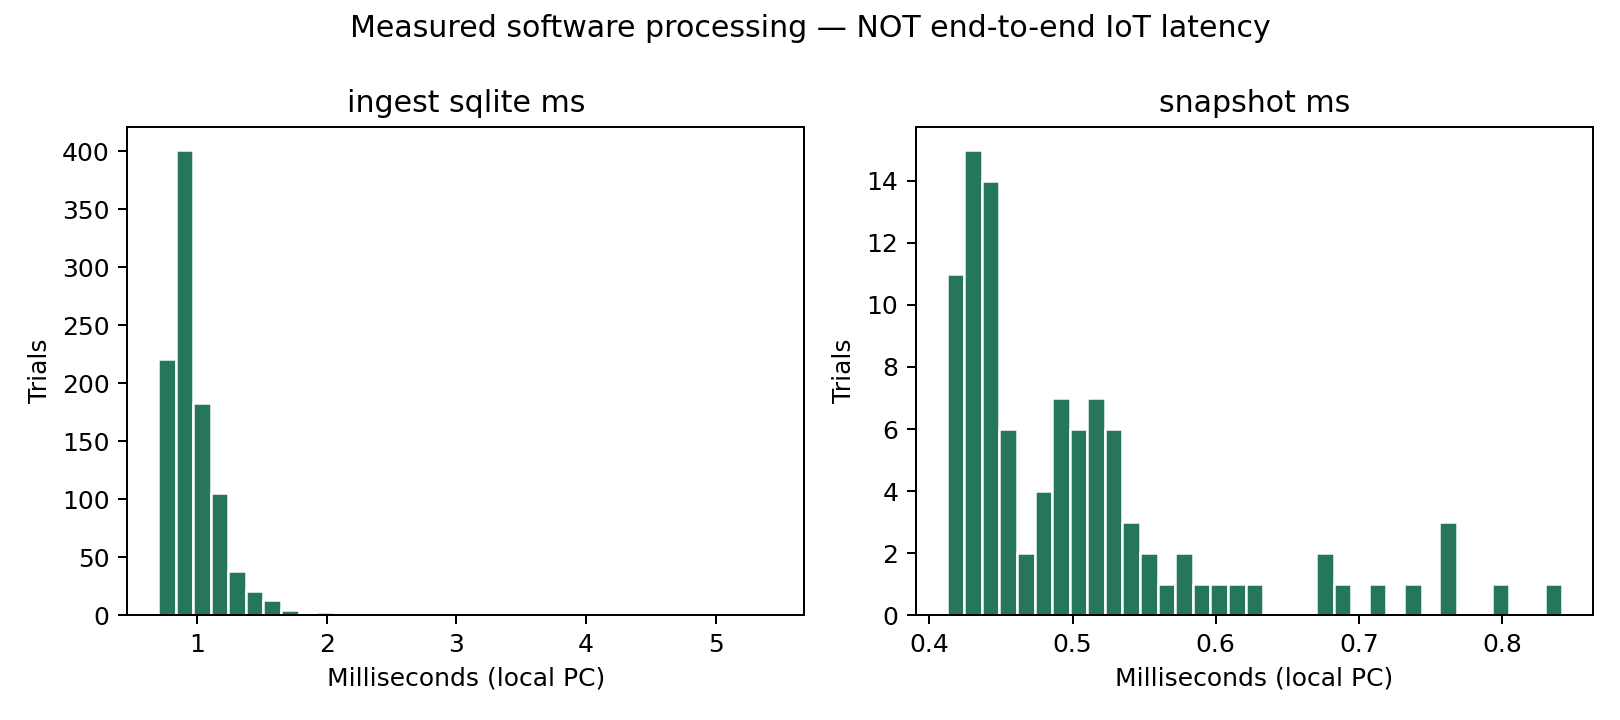
\includegraphics[width=\textwidth]{../evidence/software_latency.png}
\caption{Phân bố thời gian xử lý phần mềm thực đo, chưa bao gồm radio, Internet hoặc CoreIOT.}
\end{figure}
Thời gian thay đổi theo lịch hệ điều hành, I/O và cấu hình máy. Trung bình riêng từng khối không thể cộng để khẳng định độ trễ dashboard dưới một ngưỡng: dashboard poll mỗi giây, và USB, radio, MQTT/cloud đều có độ trễ chưa đo. Snapshot cũng không mô phỏng nhiều người dùng đồng thời.

\subsection{Lưu bền và phục hồi outbox}
Trong lượt đo, số bản tin outbox trước giả lập lỗi publish là 1.000; sau callback publish thất bại vẫn 1.000; đóng/mở database vẫn 1.000. Sau transport giả trả xác nhận thành công, flush được 1.000 và còn 0. Kết quả chứng minh tính lưu bền và điều kiện xóa trong mã local; không chứng minh broker thật đã nhận 1.000 bản tin.

Vì QoS 1 có thể phát lại, timestamp và nội dung gói được giữ; journal không tạo lại khi flush. Chưa kiểm thử mất điện bất ngờ giữa lúc ghi, ổ đĩa đầy, database hỏng hoặc giới hạn lưu trữ nhiều tháng. WAL/giao dịch không thay thế chính sách sao lưu.

\subsection{Đánh giá AI trên dữ liệu sinh}
Huấn luyện dùng \AITrainCount\ mẫu bình thường; tập kiểm thử có \AITestCount\ mẫu độc lập theo seed đã công bố. Accuracy là \AIAccuracy\%; với lớp bất thường, precision \AIPrecision\%, recall \AIRecall\%, F1 = \AIFone. Ma trận nhầm lẫn có TN=\TrueNegative, FP=\FalsePositive, FN=\FalseNegative, TP=\TruePositive.

\begin{figure}[H]\centering
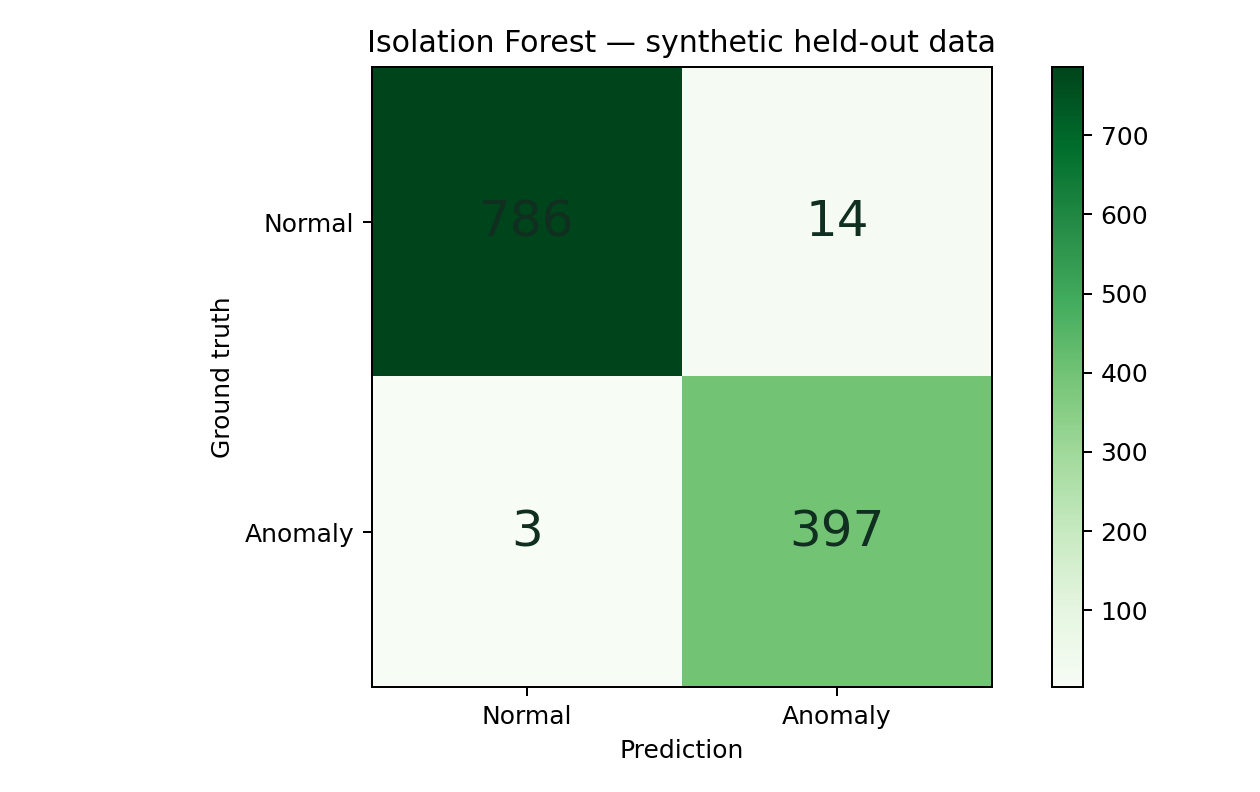
\includegraphics[width=.83\textwidth]{../evidence/confusion_matrix.png}
\caption{Confusion matrix trên dữ liệu sinh giữ riêng; không phải dữ liệu phòng học thực.}
\end{figure}
Những bất thường được sinh cách phân bố bình thường tương đối xa nên mô hình có lợi thế phân tách. Mười bốn báo động giả và ba mẫu bỏ sót trong lượt dữ liệu này cho thấy ngay cả giả thiết đơn giản vẫn có lỗi. Khi dùng phòng thật có thể có thay đổi theo giờ, vị trí cảm biến và nhiều trạng thái hợp lệ chưa có trong train. Cần giữ riêng phiên/ngày/phòng để kiểm tra tổng quát hóa, báo cáo false alarm theo thời gian và xem xét recalibration.

\subsection{Kế hoạch đo phần cứng cần bổ sung}
\begin{longtable}{P{4cm}P{7.2cm}P{3.5cm}}
\caption{Các phép đo thực tế chưa thực hiện, không điền số ước đoán}\\
\toprule Chỉ số & Cách đo và số lần đề xuất & Mục tiêu / trạng thái \\ \midrule
Sensor $\rightarrow$ dashboard & 30 lần; đánh dấu mẫu và sự kiện hiển thị bằng cùng clock/trace hoặc quay màn hình có mốc xác định; nêu rõ chu kỳ lấy mẫu/poll. & $<5$ giây; chưa đo \\
Dashboard $\rightarrow$ ACK & 30 lệnh bật/tắt, lấy thời điểm gửi và nhận ACK cùng PC; thêm quan sát/quay quạt. & $<2$ giây; chưa đo \\
Mất gói ESP-NOW & Theo từng boot, 1.000 gói ở 1/5/10 m; đối chiếu seq gửi và nhận, ghi vật cản/channel. & Ghi trung bình/min/max; chưa đo \\
Tầm truyền & Tăng khoảng cách và ghi tỉ lệ nhận, thời gian thử, môi trường; không chỉ nêu một cự ly duy nhất. & Chưa đo \\
Alert cloud/notification & Ít nhất 10 lần tạo alarm mới; ghi thời điểm phát mẫu, alarm và thông báo nhận. & Chưa đo \\
Độ chính xác cảm biến & So với thiết bị tham chiếu ở nhiều điều kiện; lặp và ghi độ lệch. & Chưa đo \\
Ổn định dài hạn & 24 giờ, ngắt USB/mạng có kịch bản, lưu số reboot và hàng đợi. & Chưa chạy \\
Công suất/OTA & Không có thiết bị đo công suất và không triển khai OTA. & Không báo số liệu \\
\bottomrule
\end{longtable}
Tỷ lệ mất gói theo một phiên có thể tính $100(N_{sent}-N_{received,unique})/N_{sent}$. Cần xác định gói đầu/cuối và số gói sender thật sự gửi, không dùng một khoảng sequence bị cắt đầu/cuối tùy ý. Không trộn nhiều boot hoặc tính gói trùng như gói mới.

\section{Đánh giá kết quả}
Các mục tiêu local về từ chối dữ liệu sai, loại trùng, hysteresis, ACK/timeout và outbox đã có test tương ứng. AI đã có mô hình, phép đo CPU và dữ liệu dự đoán truy xuất được; mức tin cậy hiện giới hạn trong dữ liệu sinh. Hai firmware đủ điều kiện bước tiếp theo là cấu hình MAC/pin và nạp thử, không phải kết luận đã vận hành ổn định.

Telemetry và RPC mô phỏng đã được xác nhận; API local ghi các RPC ID applied và outbox bằng 0. Ảnh người dùng cung cấp còn cho thấy alarm Major, New alarm notification và Alarm cleared notification, xác nhận T12/T13 ở mức chức năng với dữ liệu mô phỏng. Chưa đo lặp độ trễ sensor--cloud, notification hoặc mất gói vô tuyến; không dùng nhãn thời gian tương đối trên ảnh làm số đo độ trễ. Script cập nhật tại chỗ đã kiểm thử cục bộ, nhưng người dùng chọn tự sửa switch. Trước nộp cần lưu tệp ảnh/export cấu hình và thực hiện phép đo phần cứng còn thiếu.
